\documentclass{article}

\usepackage{corl_2026}
\usepackage{amsmath}
\usepackage{amssymb}
\usepackage{booktabs}
\usepackage{graphicx}
\usepackage{subcaption}
\usepackage{microtype}
\usepackage{xspace}

\title{Certified Predictive Reduction for Bounded-Memory Robot Uncertainty Monitors}

\author{
  Anonymous Authors\\
  Anonymous Institution\\
  \texttt{anonymous@anonymous.edu}
}

\newcommand{\pzr}{PZR\xspace}
\newcommand{\mpcg}{\textsc{MPC-G}\xspace}
\newcommand{\mpcw}{\textsc{MPC-W}\xspace}
\newcommand{\gen}{\mathrm{gen}}
\newcommand{\reduce}{\rho}
\newcommand{\concretize}{\gamma}

\begin{document}
\maketitle

\begin{abstract}
Robotic systems increasingly rely on runtime monitors to track safety-relevant
quantities computed from noisy sensor streams. Affine arithmetic gives a
principled way to distinguish persistent calibration bias from fresh
measurement noise, but the resulting zonotope representation grows with every
measurement. Existing bounded-memory monitors therefore reduce zonotopes online,
usually with a fixed geometric rule that ignores how reduction error affects
future trigger verdicts. We formulate zonotope reduction as a certified
abstraction-control problem: an untrusted predictive or learned policy chooses
among certified reducers, while reducer certificates alone preserve soundness
and the generator budget. On an omnidirectional robot monitoring benchmark, a
focused receding-horizon selector improves trigger-relevant precision over a
strong static Girard reducer at the same memory budget; a distilled neural
selector approximates expensive decisions at lower online cost while remaining
outside the trusted soundness boundary.
\end{abstract}

\keywords{Robot Monitoring, Uncertainty, Zonotopes}

\section{Introduction}

Robots act from streams of imperfect observations. Wheel odometry, inertial
measurements, range readings, and temperature or power sensors all contain
uncertainty with different temporal structure: some error is persistent
calibration bias, while other error is independent measurement noise. Runtime
monitors are an attractive tool for such systems because they can continuously
compute safety-relevant derived quantities and trigger warnings without changing
the robot controller. For embedded deployment, however, monitors must also have
a resource footprint that is independent of trace length.

Recent work on stream-based monitoring under uncertainty shows that affine
arithmetic can track these uncertainty sources symbolically and that the affine
coefficients form a zonotope~\citep{finkbeiner2026cutting}. This gives precise
semantics for monitor state, but each fresh measurement-noise variable adds a
new zonotope generator. Without approximation, memory grows forever. Classical
zonotope order reduction~\citep{girard2005reachability,yang2018comparison}
solves the bounded-memory problem by replacing a high-order zonotope with a
certified over-approximation containing fewer generators. The reduction choice
matters: losing a correlation that appears harmless at the current time can
inflate a future trigger interval after the monitor equations propagate it.

This paper treats reduction as a control decision over monitor abstractions.
When the monitor state exceeds a generator budget \(K\), a policy chooses a
reducer action \(a\) from a finite certified action set, applies only the first
chosen reduction, and replans at the next overflow. The policy can be static,
model-predictive, or learned by imitation. It is not trusted for soundness.
Soundness depends only on the reducer certificate
\[
  \concretize(Z) \subseteq \concretize(\reduce_{a,K}(Z)),
  \qquad
  \gen(\reduce_{a,K}(Z)) \le K .
\]
This separation lets us optimize monitor precision using approximate forecasts
or neural policies while keeping the runtime-assurance argument small.

Our current evidence is a research prototype and benchmark suite for predictive
zonotope reduction. The main robot benchmark is an omnidirectional monitor that
tracks filtered acceleration, velocity, distance increments, position, and
safety triggers under persistent calibration and fresh measurement uncertainty.
At budget \(K=8\), a focused rollout selector reduces mean trigger width from
230.1 to 225.1 and interval-hull mean squared error from 352.6 to 268.4 versus
the strongest static baseline, Girard. Across a budget sweep from 8 to 20
generators, the same focused selector consistently improves on Girard. The full
artifact reports zero budget violations, zero unsound certificates, and zero
reduction failures.

The contribution is threefold. First, we cast bounded-memory uncertain monitor
execution as policy-guided certified reduction, with a policy-independent
soundness argument. Second, we instantiate the idea with a focused
receding-horizon selector that scores future trigger precision while preserving
monitor-required calibration generators. Third, we distill expensive selector
decisions into a neural policy and evaluate the current tradeoff: faster
decisions and preserved certificates, but not yet a stronger precision result
than focused rollout.

\section{Related Work}

\textbf{Runtime monitoring for robotic and cyber-physical systems.}
Stream-based monitoring languages such as Lola and RTLola describe monitors as
stream transformations whose outputs include trigger verdicts. RTLola emphasizes
static analyses for bounded memory and runtime safety, and has been used in
autonomous-aircraft monitoring~\citep{baumeister2020cleared,baumeister2026rtlola}.
The uncertainty-aware monitor semantics of \citet{finkbeiner2026cutting}
replace exact stream values by affine forms, giving a symbolic account of
calibration and measurement uncertainty. Our work keeps this semantic stack but
changes the online approximation-selection step.

\textbf{Zonotopes and set-based estimation.}
Zonotopes are widely used in reachability analysis, set-membership estimation,
and fault diagnosis because they are compact and closed under linear maps and
Minkowski sums~\citep{girard2005reachability,combastel2003state}. The practical
limitation is order growth, so many reduction rules have been proposed and
compared~\citep{kopetzki2017methods,yang2018comparison}. These methods normally
optimize present-set geometry or generic enclosure size. We instead choose
among certified reductions using a monitor-aware future cost, so the objective
is trigger precision after stream equations propagate the approximation.

\textbf{Predictive and learned control.}
Our selector borrows the receding-horizon pattern from model predictive
control~\citep{rawlings2009mpc}: optimize over a finite forecast, apply the
first decision, and replan. The controlled variable here is not an actuator but
a compression action. Learning enters as policy distillation. Imitation learning
can replace expensive expert decisions with cheap policies
\citep{ross2011dagger}; in our setting, the learned model never justifies
soundness, because every proposed action is still checked by a certified
reducer.

\section{Policy-Guided Certified Reduction}

\subsection{Monitor State}

Let an uncertain monitor state be represented by a zonotope
\[
  Z = c + G[-1,1]^m,
\]
where \(c\) is the nominal vector of monitor stream values and each column of
\(G\) is a symbolic uncertainty generator. Persistent calibration errors reuse
generators across time, while fresh measurement noise appends new generators.
The exact affine monitor transition is assumed sound: stepping the monitor over
an uncertain state over-approximates all concrete executions represented by the
input state. The difficulty is that \(m\) grows with trace length.

A bounded-memory monitor imposes a budget \(K\) on stored generators. A reducer
action \(\reduce_{a,K}\) is admissible only when it returns a certificate that
establishes both enclosure and budget:
\begin{equation}
  \concretize(Z) \subseteq \concretize(\reduce_{a,K}(Z)),
  \qquad
  \gen(\reduce_{a,K}(Z)) \le K .
  \label{eq:contract}
\end{equation}
The implementation includes box, Girard, Combastel, transform-based, PCA,
adaptive, and scored keep-and-box reducers. A protected wrapper preserves
monitor-required generators, such as calibration variables, exactly before
compressing the residual zonotope.

\subsection{Policy-Independent Soundness}

The policy is a selector
\[
  \pi_t : H_t \times Z_t \times \widehat{x}_{t:t+h} \rightarrow A,
\]
where \(H_t\) is observed history, \(Z_t\) is the current monitor state,
\(\widehat{x}_{t:t+h}\) is an optional predicted input trace, and \(A\) is a
finite reducer set. If \(Z_t\) exceeds budget, the monitor applies
\(\reduce_{\pi_t,K}\). The policy may be static, predictive, learned, or
suboptimal; it is sound as long as it cannot bypass Eq.~\eqref{eq:contract}.

\textbf{Proposition.}
Assume the unreduced monitor transition soundly encloses all concrete states
represented by its input zonotope. If every applied reducer satisfies
Eq.~\eqref{eq:contract}, then the reduced monitor execution over-approximates
the unreduced affine execution at every step. Moreover, every stored
post-reduction state has at most \(K\) generators.

The proof is by induction over monitor steps. Monitor transitions preserve
sound enclosure by assumption. Reduction steps preserve enclosure by the
certificate, independently of how the reducer action was selected. The budget
invariant follows directly from the second part of Eq.~\eqref{eq:contract}.

\subsection{Predictive and Learned Selectors}

The focused rollout policy, \mpcg, evaluates a small protected action set for
the first reduction. For each candidate it rolls the monitor forward over a
short input forecast, reducing future predicted overflows with protected Girard
and an emergency protected box fallback. It scores future states by
trigger-relevant interval width and threshold straddling, applies only the best
first action, and replans at the next real overflow.

We also evaluate a broader rollout ablation, \mpcw, whose first-action set
includes more static protected reducers. This tests whether simply widening the
action set helps. In the current artifact it does not: the broad selector is
slower and less precise on the hard robot than \mpcg.

Finally, we train a small neural classifier from logged selector decisions. At
runtime the learned policy ranks reducers, then tries them in that order until a
certified budgeted reduction succeeds. If the top prediction fails the
certificate or budget check, it is skipped. Thus learning affects precision and
latency, not soundness.

\section{Experiments}

\subsection{Setup}

The evaluation uses three monitor families. The headline scenario is an
omnidirectional robot monitor with persistent calibration uncertainty and fresh
measurement noise. It tracks filtered acceleration, velocity, distance
increments, and \(x/y\) position, then evaluates interval trigger verdicts. We
also include a simpler two-axis robot monitor and a thermostat monitor as
sanity checks outside the main robot setting.

The main run uses 50 seeds, trace length 300, generator budget \(K=8\), horizon
6, and both online and oracle predictors. Unless stated otherwise, we report
online results. Metrics compare bounded monitors against an unreduced reference
execution. Lower trigger width, width inflation, false-alarm rate, and
interval-hull MSE are better. The unbounded reference is not a deployable
bounded-memory baseline.

\subsection{Hard Robot Results}

Table~\ref{tab:robot} gives the main online comparison on the
omnidirectional robot. Girard is the strongest static bounded-memory baseline.
\mpcg improves both mean trigger width and width inflation at the same mean
generator count. Its runtime is roughly ten times Girard because it performs
rollout search. The learned selector is faster than rollout and close to Girard
precision, but it does not match \mpcg on the main precision metric.

\begin{table}[t]
  \centering
  \caption{Online omnidirectional robot results at budget \(K=8\), horizon 6,
  length 300, and 50 seeds. Lower is better except mean generators, which
  indicates budget usage.}
  \label{tab:robot}
  \begin{tabular}{lrrrrr}
    \toprule
    Method & Trigger width & Hull MSE & False alarm & Time (s) & Mean gen. \\
    \midrule
    Girard & 230.1 & 352.6 & 0.0105 & 0.098 & 7.93 \\
    \mpcg & \textbf{225.1} & \textbf{268.4} & 0.0113 & 0.957 & 7.93 \\
    \mpcw & 242.5 & 728.6 & 0.0127 & 2.533 & 7.74 \\
    Learned & 229.2 & 332.2 & 0.0115 & 0.169 & 7.92 \\
    \bottomrule
  \end{tabular}
\end{table}

The budget sweep in Fig.~\ref{fig:robot_budget} is the cleanest evidence that
the predictive choice matters. \mpcg has lower interval-hull MSE than Girard
for all evaluated budgets from 8 to 20 generators. The broad rollout ablation
is worse despite evaluating more candidates, suggesting that monitor-aligned
action design matters more than action-set size.

\begin{figure}[t]
  \centering
  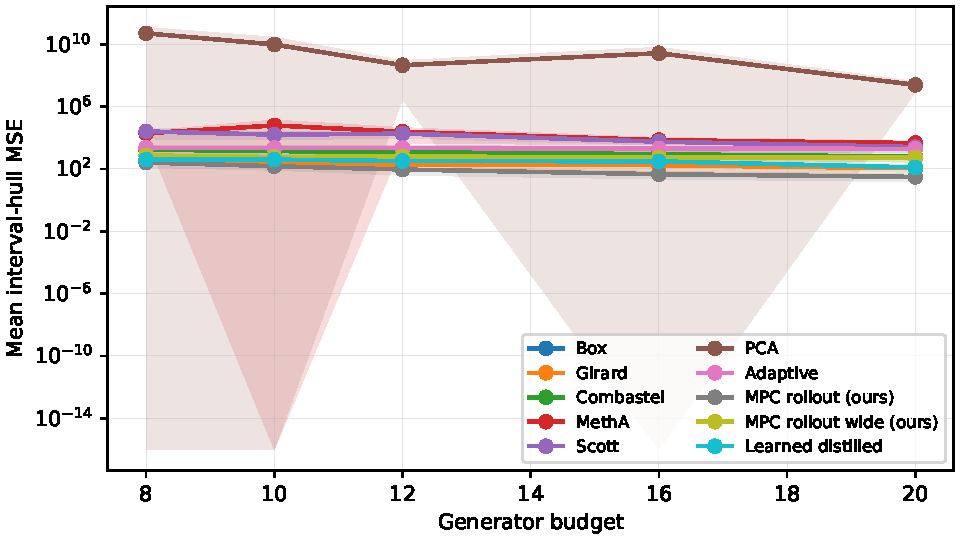
\includegraphics[width=0.86\linewidth]{figures/fig5b_omni_error_by_budget.pdf}
  \caption{Omnidirectional robot interval-hull MSE by generator budget. The
  focused rollout selector improves over Girard across the evaluated budget
  range.}
  \label{fig:robot_budget}
\end{figure}

Figure~\ref{fig:robot_time} shows error over time at the default budget. The
gap grows along the trace, matching the intuition that local approximation
choices compound through future monitor equations.

\begin{figure}[t]
  \centering
  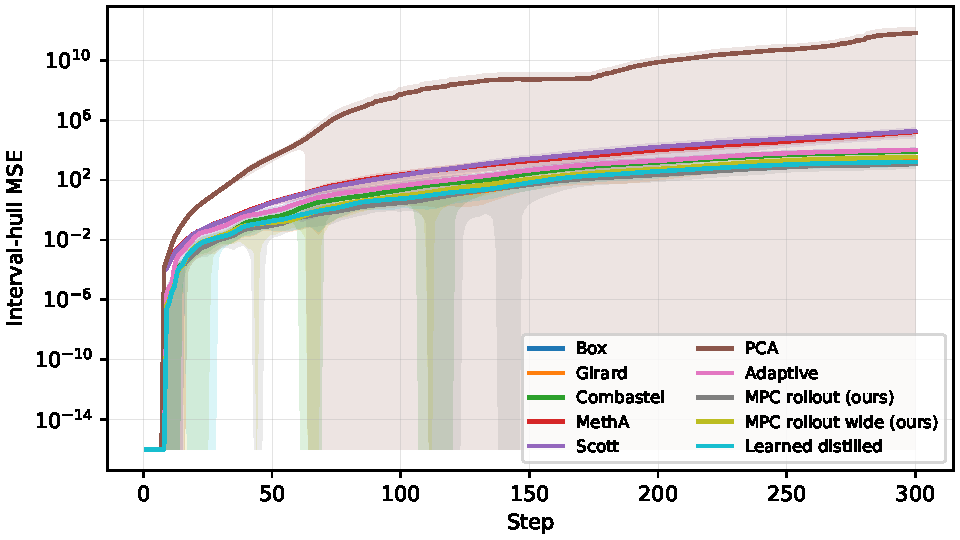
\includegraphics[width=0.86\linewidth]{figures/fig5a_omni_error_over_time.pdf}
  \caption{Omnidirectional robot error over time at the default budget.}
  \label{fig:robot_time}
\end{figure}

\subsection{Diagnostics and Learning}

The artifact reports zero budget violations, zero unsound certificates, and
zero reduction failures over 3300 aggregate run rows. This is the empirical
check for the formal boundary: all state-changing decisions passed through
certified reducers.

Selector diagnostics explain the method behavior. On the robot, \mpcg selects
protected Girard for most reductions with occasional keep-generator choices.
\mpcw uses a broader first-action distribution but pays higher decision cost
and produces worse robot precision. The learned model is trained on 40,862
decision rows to imitate the broad rollout expert. Validation accuracy is
90.6\% and top-3 accuracy is 98.8\%, but the label distribution is highly
imbalanced toward Girard. We therefore treat distillation as a safe acceleration
path rather than a standalone learning result.

The simple robot and thermostat monitors are useful checks that the certified
boundary and artifact pipeline work beyond one scenario. They are not the main
evidence for dominance: several certified reducers saturate their trigger-width
metrics near the reference.

\section{Limitations}

The current evidence is not yet a complete CoRL robotics story. The robot
scenario is a simulation benchmark for a monitor, not a deployed robot system.
Future work should evaluate on logged or live robot traces where monitor
verdicts affect runtime assurance decisions. The auxiliary non-robot scenarios
are too easy under the current configuration, so they mainly test generality of
the implementation rather than precision improvements.

The learned selector is also preliminary. Its expert labels are imbalanced and
mostly teach a Girard-heavy shortcut. A stronger learning contribution should
train against the focused expert, rebalance rare actions, or use expert
iteration so the policy can improve the precision/runtime frontier rather than
only imitate it. Finally, the online predictor is simple; robust or tube-aware
prediction may matter on traces where oracle forecasts create a larger gap.

\section{Conclusion}

Bounded-memory uncertainty monitors need reduction, but reduction need not be a
fixed local rule. We presented policy-guided certified zonotope reduction, where
predictive and learned policies optimize precision while certified reducers
preserve soundness and memory bounds. Current results support a focused claim:
receding-horizon reduction improves precision on a hard robot monitor at the
same generator budget, and learned selectors can be placed outside the trusted
soundness boundary. The next step is to turn this monitor benchmark into a
robotics-facing evaluation with richer traces and stronger learned policies.

\clearpage
\acknowledgments{Omitted for anonymous submission.}

\bibliography{references}

\end{document}
